\chapter{Methodology}

This section describes the data workflow from preprocessing to evaluation and the tools we used at each step. We designed our workflow into four stages:
\begin{itemize}
    \item preprocessing and slide level data processing
    \item selection of valid spectra
    \item training models and synthetic data generation
    \item evaluation under the TS/TR and TSR/TR regimes against the baseline TR/TR
\end{itemize}

\section{Data Collection}

We analyzed the dataset of glioma RS biopsies collected for the study performed by Lita et al. [cite]. The data acquizition protocol is described in detail in their study. The biological samples and the corresponding methylome labels were provided by Dr. Houtan Noushmehr; the samples were collected at the Hermelin Brain Tumor Center at Henry Ford Health System. The samples were anonymized and all the patients consented to have their acquired data used for research purposes.

The resulting dataset consists of ~270,000 Raman spectra from 59 biopsy scans. For data quality reasons, we used only 58 samples. Each sample scan is a $(H_i,W_i,N_\lambda)$ tensor, with $H_i$ and $W_i$ the width and height of the slide $i$, in number of pixels, and $N_\lambda = 1738$ represents the number of spectral bands or spectral dimension, which is constant throught the dataset as all of the samples were processed with the same spectrometer.

The samples are labeled with LGm1 to LGm6, corresponding to 6 distinct methylation profiles. The labels (LGm1, LGm2, LGm3) are all classified as IDH-mutant tumour, while the labels (LGm4, LGm5, LGm6) are classified as IDH-wildtype. This coarser classification is very impotrant, as it corresponds to a much higher physiological difference than the differences between methylation profiles. This allows us to formulate two problems, one of binary classification of tumour grade between mutant and wildtype and a more difficult problem of determining the methylation profile. The number of samples per class can be found in Table \ref{tab:dataset}

\begin{table}[h]
\centering
\caption{Number of samples by tumor grade class.}
\label{tab:dataset}
\begin{tabular}{llcc}
\toprule
\textbf{Methylation} & \textbf{IDH Group} & \textbf{No. of Slides} & \textbf{No. of Slides Group} \\
\midrule
LGm1 & Mutant   & 5   \\
LGm2 & Mutant   & 12 & 26 \\
LGm3 & Mutant   & 9   \\
\midrule
LGm4 & Wildtype & 13  \\
LGm5 & Wildtype & 15 & 33\\
LGm6 & Wildtype & 5   \\
\bottomrule
\end{tabular}
\end{table}

\subsection{Cross Validation design}
For rigurous results, we want to implement a Cross Validation (CV) scheme. Standard CV divides the samples into N subsets of approximately equal size that form a partition of the dataset. Training is performed on N-1 subsets and testing on the subset left out of the training phase. In more complex settups where the classes are imbalanced, the CV split needs to be performed stratified by class to ensure that all classes are represented in each CV split. In cases where some classes are severely underrepresented, like the LGm1 and LGm6 classes, a standard CV split might be impossible to acheive. In our case, we aim to perform a 5 fold CV split at patient level. Out of the 5 samples of class LGm6, some belong to the same patient, which makes a standard CV split impossible. However, we can relax the requirements a bit without losing the rigour of data splitting. We can drop the requirement that the split forms a partition, but keep the train-test separated at patient level for all folds. This is the CV design used by Lita et al. The full detailed CV split can be found in the Appendix.

\section{Data Preprocessing}

An important first step in data processing is separating the useful signal from the noisy measurements. We would like to seprate the tumor spectra from the healthy tissue or non-tissue measurements. As each spectrum corresponds to a pixel on the biopsy slide, it is possible that some pixels do not contain tissue and that the laser probe hit the plate material. A lot of slides appear to have some spots where there is no tissue [Insert some images]. In the absence of a ground truth labeling, we must rely on unsupervised techniques. In previous studies various techniques have been proposed [TO DO: find literatury preprocessing techniques for RS in oncology]. For example in the study by Lita et al. on this dataset they proposed the use of PCA followed by DBSCAN on all spectra. We decided to take a more conservative approach and to make the decision per slide, and to visually inspect the clusterings to double check the results. The proposed annotation pipeline consists of the following steps:

\begin{figure}[h]
    \centering
    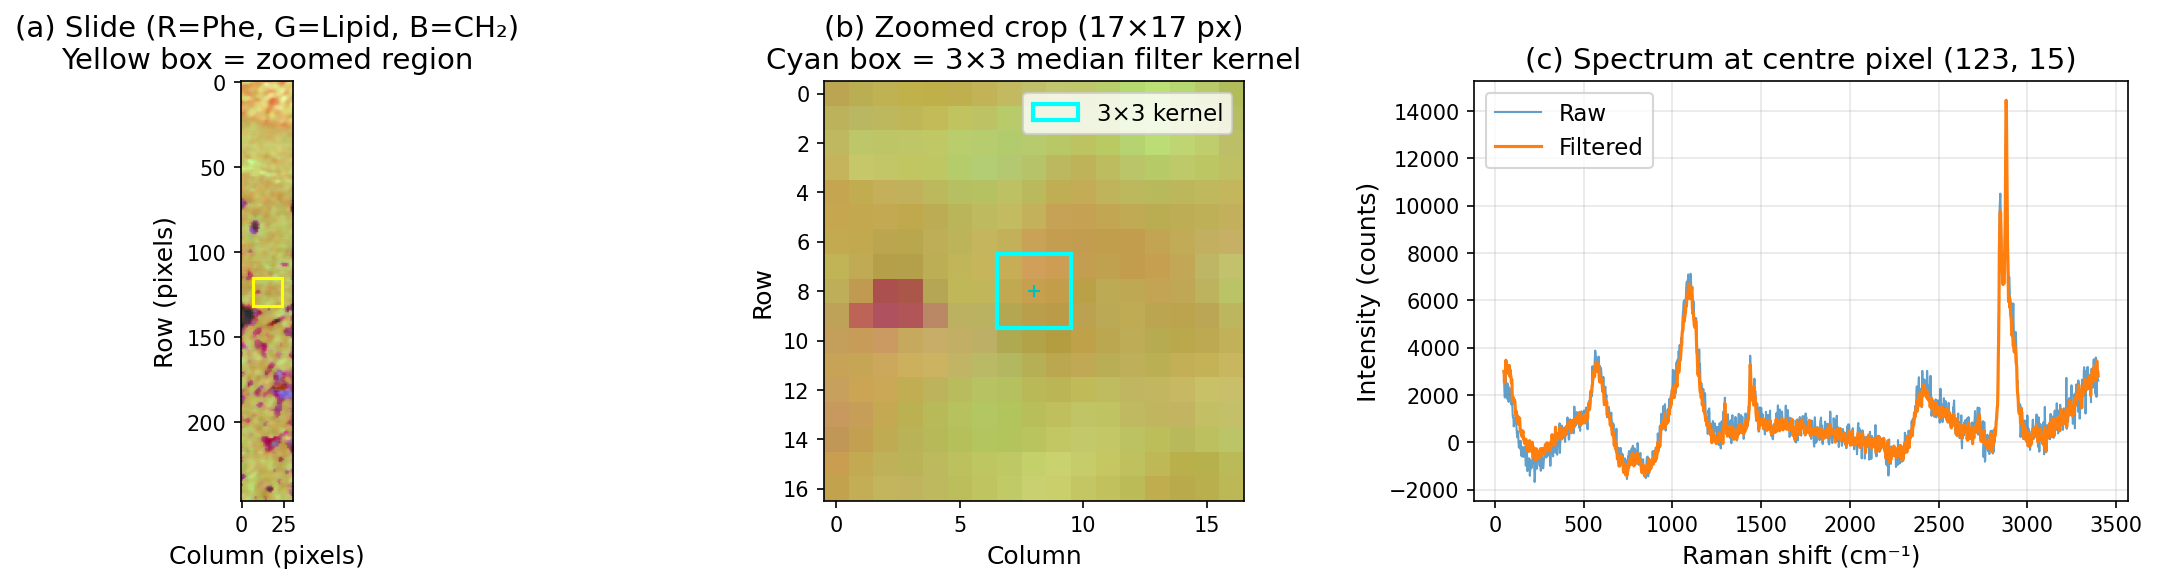
\includegraphics[width=\linewidth]{images/preprocessing_median_filter_illustration.png}
    \caption{\footnotesize (a) False coloring of a slide, with Red = Phenylalanine marker (990--1020 $\text{ cm}^{-1}$), Green = Lipids (2800--3000 $\text{ cm}^{-1}$), Blue = $CH_2$ deformations (1430--1460 $\text{ cm}^{-1}$). (b) Zoomed region for $3\times 3$ median kernel visualization. (c) Raw vs. Median filtered spectra.}
    \label{fig:preprocessing_median_filter_illustration}
\end{figure}

\begin{enumerate}
    \item \emph{Median filtering.} A $3 \times 3$ median kernel was applied on the spatial dimensions $(H,W)$ of each slide for denoising purposes, filtering out cosmic radiation and Gaussian noise (See Fig. \ref{fig:preprocessing_median_filter_illustration}). More specifically, given a position $(i,j)$, and a raw slide $S$ of size $(H,W,N_\lambda)$, let $S(i,j,l)$ be the value of the spectral band $l$ at position $(i,j)$. Then the median filtered spectral band $l$ at position $(i,j)$ is 
    $$ \text{median}(S(i,j,l)) = \text{median} \left( \left( S(\hat{i}, \hat{j}, l) \right)_{\hat{i}, \hat{j}} : \hat{i} \in \overline{i-1:i+1}, \hat{j} \in \overline{j-1:j+1} \right) $$

    \item \emph{Slide-wise normalization.} Each data tensor was normalized independently to the $[0,1]$ range to ensure numerical stability. We note that this means the entire tensor is divided by the maximum value of the tensor.

    \item \emph{Signal filtering.} We applied a simple signal quality filter by removing spectra with low intensity, setting a threshold of 0.6 on the maximum intensity of the spectrum. This step eliminates spectra that are likely dominated by noise or background, as they typically have low overall intensity. We plotted a histogram of the maximum intensity values across all spectra per slide and observed that most of the spectra have a maximum intensity close to 1, while a small subset of spectra was below the fixed threshold, hence considered low quality and removed from the dataset. Our threshold choice is rather conservative; from the maximum intensity histograms, it can be observed that a higher threshold can be selected (see Fig. \ref{fig:preprocessing_cluster_spectra} e, f).

    \item \emph{Spectral dimensionality reduction.} 

    Non-negative Matrix Factorization (NMF) \cite{NMF1999} was applied independently to each slide to obtain a lower-dimensional, non-negative representation of the spectra. NMF has previously been used in Raman spectroscopy for spectral unmixing and feature extraction \cite{NMF1999,nmf_oncology_2022, Alix2022}. We used an NMF with 100 components, as it offered sufficient reconstruction for the purpose of signal separation. 
    
    \item \emph{Gaussian Mixture Model (GMM).} A 3-component Gaussian Mixture Model (GMM) was fitted to the coefficients obtained in the previous step. We then visually inspected the clustering and selected the spectra corresponding to the components with the strongest signal. In cases where more than one cluster had similar quality spectra, and the clusters were not spatially separated in distinct regions, we selected all of them as valid spectra. This is why we refer to our pipeline as spatio-spectral as we visually analyze the clusters in both the spectral domain and the spatial domain.
    

\begin{figure}[h]
    \begin{minipage}[b]{\linewidth}
    \centering
    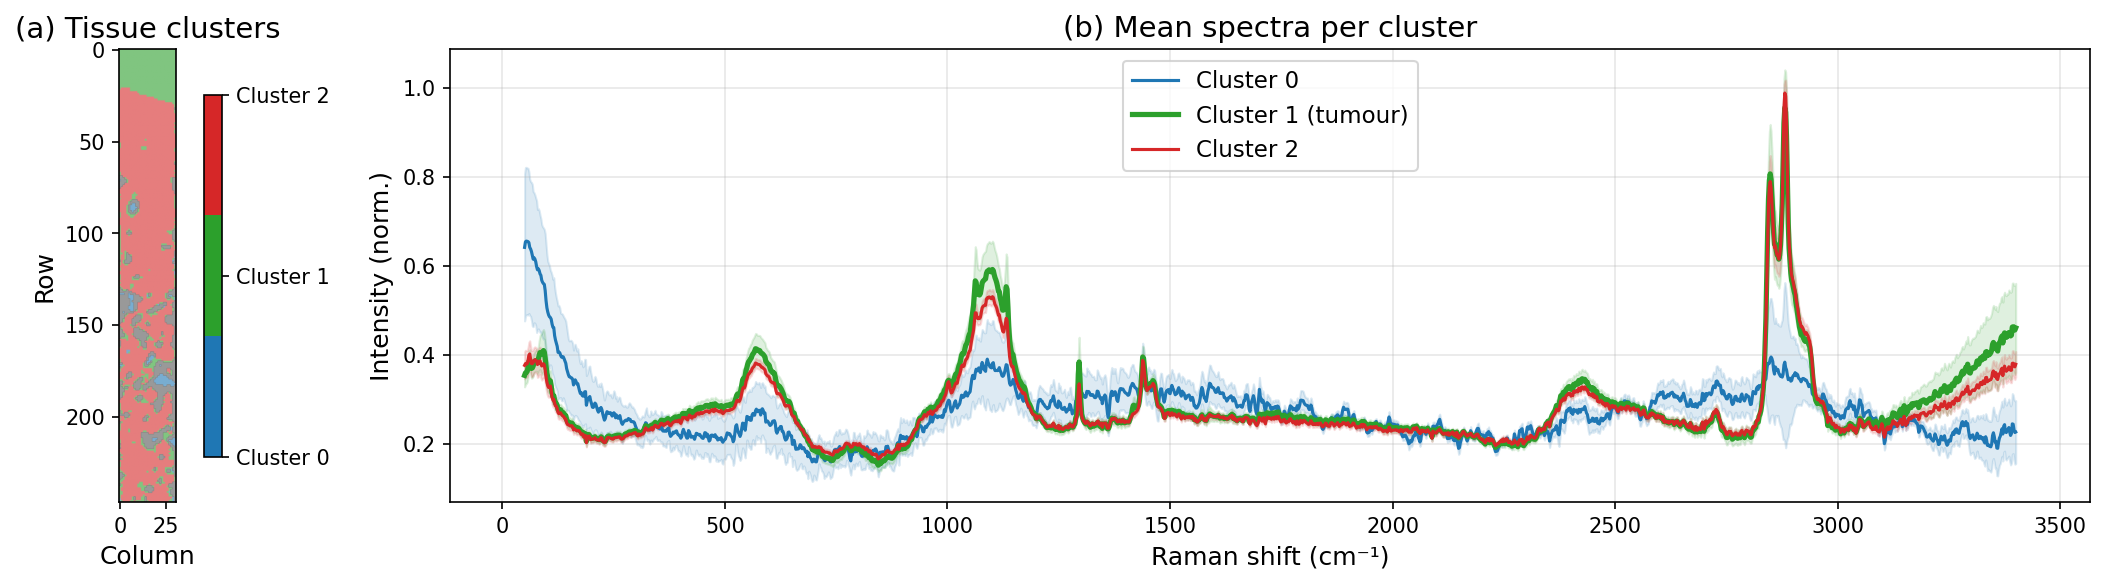
\includegraphics[width=\linewidth]{images/preprocessing_cluster_spectra.png} 
  \end{minipage}\\
  \begin{minipage}[b]{\linewidth}
    \centering
    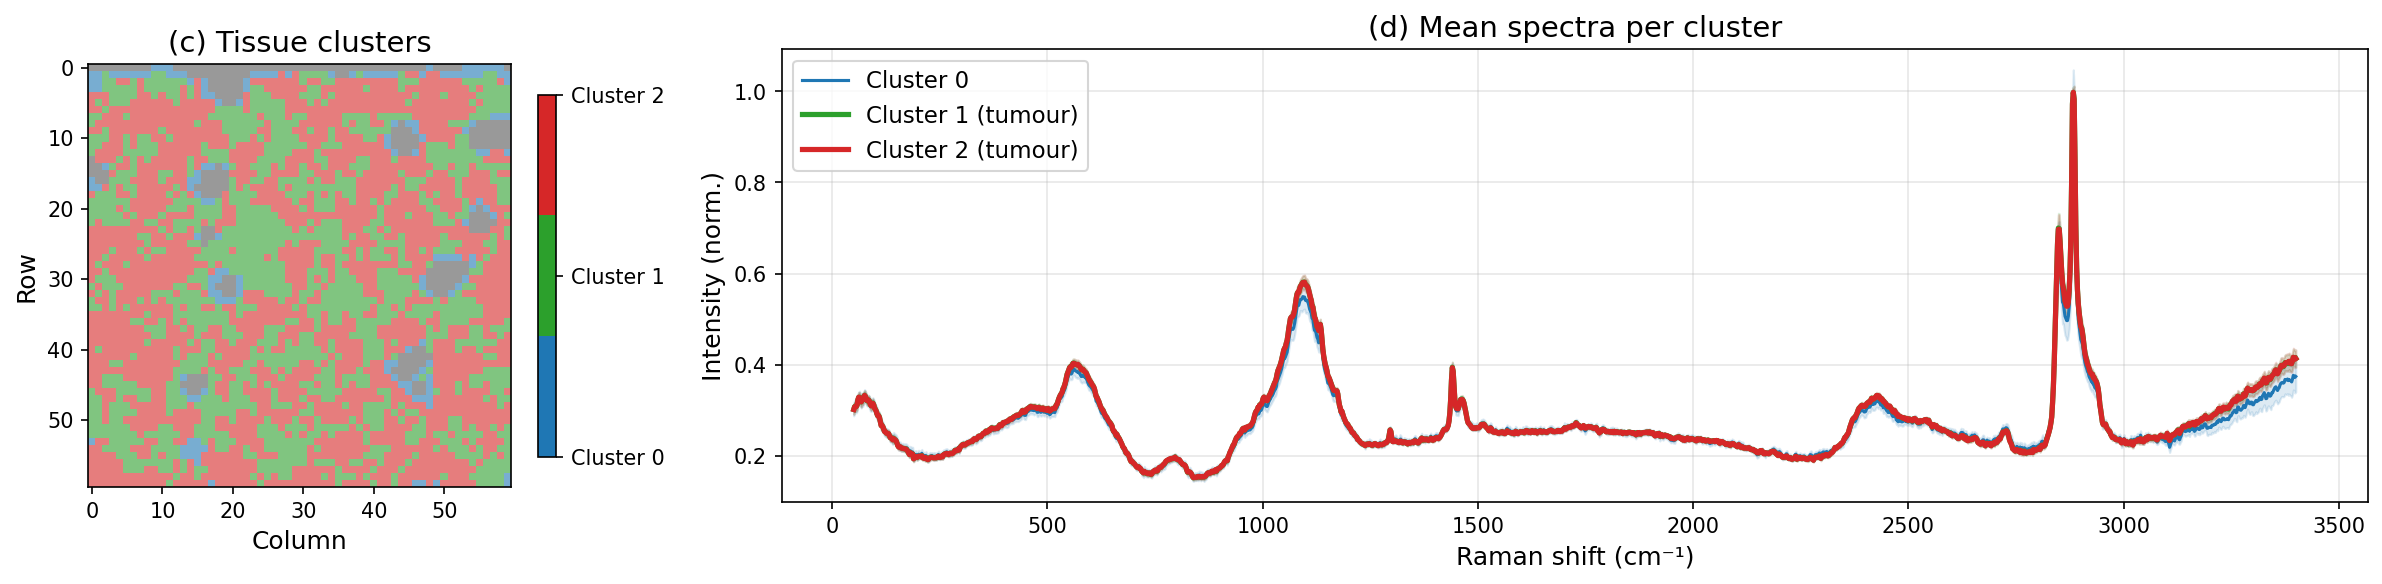
\includegraphics[width=\linewidth]{images/preprocessing_cluster_spectra_2.png} 
  \end{minipage}\\
  \begin{minipage}[b]{0.5\linewidth}
    \centering
    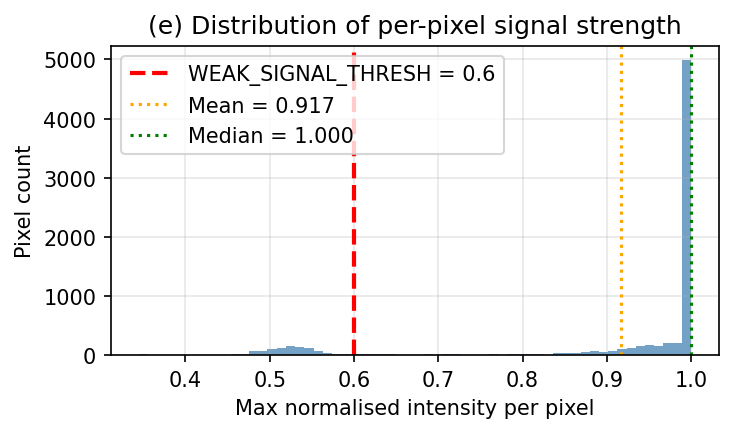
\includegraphics[width=\linewidth]{images/max_vals_distribution_img_0.png}
    \vspace{1ex}
  \end{minipage}%% 
  \begin{minipage}[b]{0.5\linewidth}
    \centering
    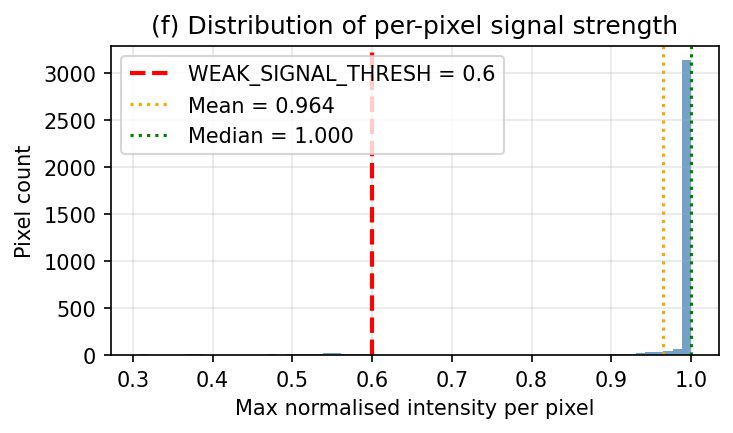
\includegraphics[width=\linewidth]{images/max_vals_distribution_img_5.png} 
    \vspace{1ex}
  \end{minipage}    
    \caption{\footnotesize Spectral clustering of two slides (top, middle). (a) Slide 1 cluster assignment; (b) Slide 1 Mean spectra per cluster: blue = weak signal cluster, discarded, red = medium intensity signal, discarded, green = strong signal, selected as tumor; (c) Slide 2 cluster assignment; (d) Slide 2 Mean spectra per cluster: red, green = strong tissue signal, selected as tumor, blue = weak signal, discarded; (e, f) Histograms of maximum intensity of spectra for the first and second slides, respectively.}
    \label{fig:preprocessing_cluster_spectra}
\end{figure}


    \item \emph{Per spectrum preprocessing.} For the spectra selected as relevant, we performed the following per spectrum processing steps: (i) [0, 1] normalization; (ii) airPLS with $\lambda=100$ and porder $p=1$; 
    

    \item \emph{Saving spectra.} We saved the processed spectra to an HDF5 file for further ML tasks. Note that we used NMF only for clustering, but the processing for saved spectra was $3 \times 3$ median filtering followed by airPLS baseline correction. We preferred to keep as much of the signal as possible, and also to keep the preprocessing simple and reproducible. The NMF reconstruction smothes the signal further, and we prefer to not compress the signal further at this point.

\end{enumerate}

\begin{figure}[h]
    \centering
    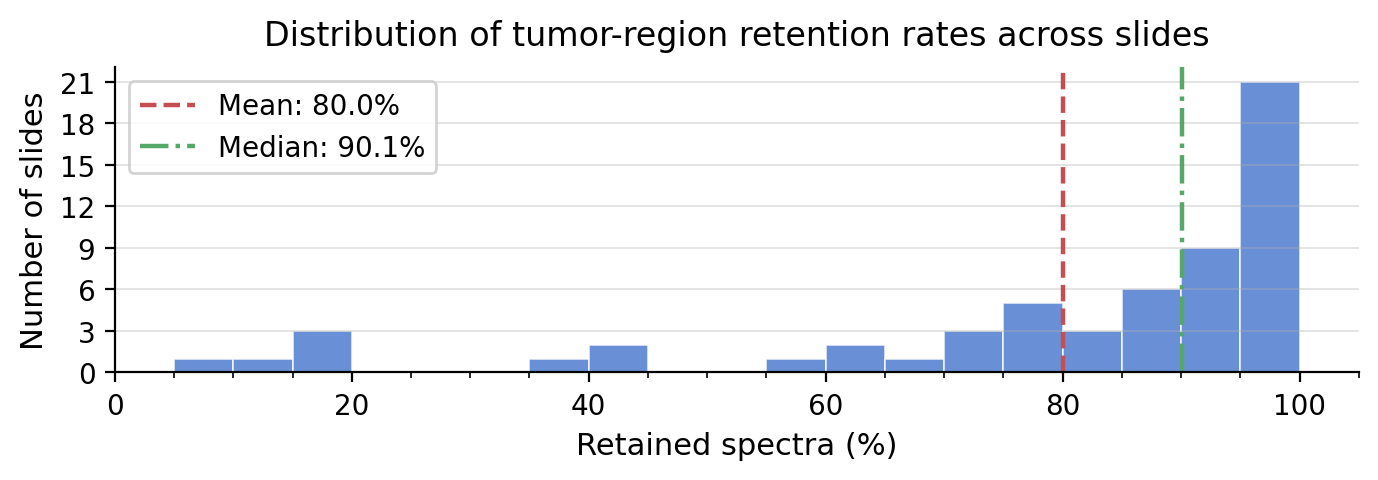
\includegraphics[width=\linewidth]{images/tumor_retention_histogram.png}
    \caption{Histogram of retention rates.}
    \label{fig:tumor_retention_rates}
\end{figure}

This approach ensured that each slide was processed independently and visually inspected to verify cluster consistency. The resulting binary tumor labeling yields approximately 200,000 spectra retained for downstream analysis from the original $\sim$270,000. We draw attention to the fact that the percentage of retained spectra from each slide varied significantly (see Fig. \ref{fig:tumor_retention_rates}). We note that the two step filtering of viable pixels, via a maximum intensity threshold followed by clustering has some degree of robustness; low signal quality spectra not filtered by the threshold will be filtered by the clustering and manual selection. On the other hand, as noted earlier, this pipeline is not standard or unique, but applies some common data processing techniques to the given problem under assuptions like spatial cohesiveness or spectral similarities.


\section{Deep Generative Augmentation}
\label{sec:cvae_architecture}
To learn the underlying distribution of tumor spectra, we implemented a 1D-Convolutional Conditional Variational Autoencoder ($\beta$-CVAE). 1D convolutions were chosen to exploit the strong local dependencies between adjacent Raman shift frequencies (e.g., the broad lipid/protein bands between $1400$ and $1500 \text{ cm}^{-1}$). 

As illustrated in Figure \ref{fig:cvae_architecture}, the architecture is composed of an encoder, a $d$-dimensional latent bottleneck, and a decoder. The encoder $q_\phi(z|x)$ compresses the input Raman spectrum $x$ into a latent representation $z$. To encourage class separation in the reconstructed spectra, $\hat{x}$, we conditioned the decoder $p_\theta(\hat{x}|z,y)$ on the class label $y$ provided as a one-hot encoded vector. 

To ensure that the encoder learns class discriminative features, we framed the encoding process as a Multi-Task Learning (MTL) problem by appending an auxiliary classification head to the encoder.
The model is optimized using a composite loss function:
\begin{equation}
\mathcal{L}_{\text{total}} = \mathcal{L}_{\text{recon}} + \beta \cdot D_{KL}(q_\phi(z|x) \| p(z)) + \alpha \cdot \mathcal{L}_{\text{class}}. 
\end{equation}

$\mathcal{L}_{\text{recon}}$ represents the reconstruction loss, and is defined as
\begin{align}
\mathcal{L}_{\text{recon}} &= \gamma \cdot \text{MSE}(x, \hat{x}) + (1 - \gamma) \cdot \text{CosineLoss}(x, \hat{x}) \\
\nonumber &= \gamma \cdot \frac{1}{N_{\lambda}} \| x - \hat{x} \|_2^2 + (1 - \gamma) \cdot \left(1 - \frac{x \cdot \hat{x}}{\|x\|_2 \|\hat{x}\|_2}\right). 
\end{align} 
We performed multiple experiment and we tested with values of $\gamma \in \{0, 0.5, 1\}$.

$\mathcal{L}_{\text{class}}$ represents the categorical cross-entropy loss of the auxiliary classifier: 
\begin{equation}
\mathcal{L}_{\text{class}} = - \sum_{c=1}^{C} y_c \log(p_c),
\end{equation} where $y_c$ is the true label and $p_c$ the predicted probability associated with class $c$. The categorical cross-entropy loss is scaled by $\alpha$; in our experiments, we set $\alpha \le 0.5$ empirically, as the classification task is auxiliary and included only for training the encoder. We observed that scaling by a factor $\alpha = 0.5$ led to overfitting the encoder on the classification task very early during training, therefore we chose $\alpha = 0.2$ which led to a similar rate of convergence across the classification and the reconstruction tasks.

The parameter $C \in \{2, 6\}$ denotes the number of label classes, $C=2$ for binary classification (IDH-mutant, IDH-wildtype), or $C = 6$ for classifying all six glioma sub-types.

Once trained, the decoder can generate class-balanced synthetic datasets
by sampling $z \sim \mathcal{N}(0, I)$ conditioning on a requested class label.

\begin{figure}[h]
    \centering
    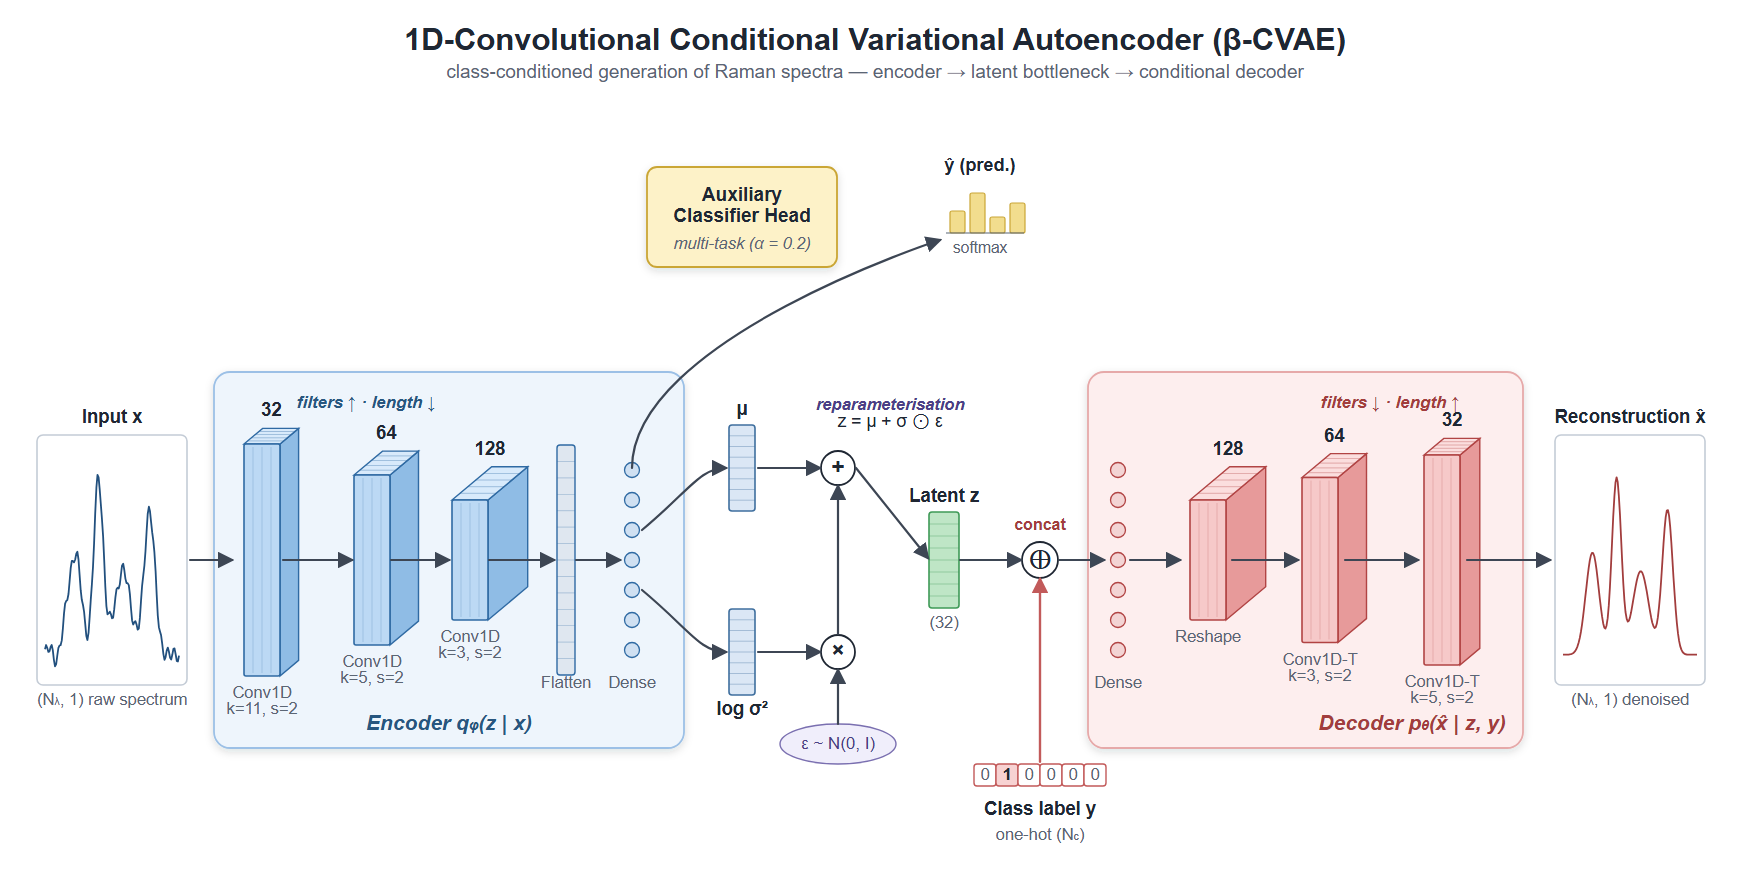
\includegraphics[width=\linewidth]{images/cvae_architecture.png}
    \caption{\footnotesize Architecture of the 1D-Convolutional Conditional Variational Autoencoder ($\beta$-CVAE). The encoder is composed of 1-d convolutional layers with 3 blocks: filters $[32, 64, 128]$, kernels $[11, 5, 3]$, and strides $[2, 2, 2]$, compressing the input spectrum to the $d$-dimensional latent space. The decoder reconstructs the spectrum conditioned on both the latent representation and the class label, using transpose convolutions with initial filters of 128, followed by 3 blocks with filters $[128, 64, 32]$, kernels $[3, 5, 11]$, and strides $[2, 2, 2]$. 
    %The model is trained with batch size 256 for 70 epochs at learning rate $0.001$ with reconstruction loss mode MSE, generating 20,000 samples per class.  
    An auxiliary classifier head is attached to the encoder to encourage the convolutional layers to capture class discriminative features.}
    \label{fig:cvae_architecture}
\end{figure}

Following the $\beta$-VAE framework introduced by Higgins et al. \cite{higgins2017betavae}, the Kullback-Leibler divergence ($D_{KL}$) acts as a structural regularizer when scaled by $\beta>1$. 

For a Gaussian distribution regularizer, the divergence has the following expression \cite{higgins2017betavae, Asperti2020}:
\begin{equation}
D_{KL}(q_\phi(z|x) \| p(z)) = \frac{1}{2} \sum_{i=1}^{d} \left( \mu_i^2 + \sigma_i^2 - \log(\sigma_i^2) - 1 \right).
\end{equation}

According to Higgins et al., a higher weight for the divergence term ensures that the latent space is sufficiently regularized, which constitutes a requirement for the generator to be used by sampling from a normal distribution \cite{higgins2017betavae}, hence we set $\beta=2$. The latent vector $z \in \mathbb{R}^d$ has two $d$-dimensional parameters associated: $\mu$ and $\log(\sigma^2)$. In our experiments, we tested $d \in \{ 16, 32, 64 \}$, but most of the experiments used $d=32$.


\section{Classification by Reconstruction}
\label{sec:cbr}


Standard discriminative models such as Random Forests and XGBoost optimize class-separating decision boundaries from labeled training data. However, in small-cohort Raman spectroscopy settings, these models may generalize poorly to unseen samples affected by acquisition variability and changing spectrometer baselines. Motivated by this limitation, we investigate an alternative generative inference strategy, termed Classification by Reconstruction (CbR).

CbR leverages the CVAE's learned latent representations to classify a tumor without relying on discriminative boundaries. 
During inference on a preprocessed unseen test spectrum $x_{\text{test}}$, we defined the following approach:
\begin{enumerate}
    \item \emph{Latent extraction.} The test spectrum is passed through the encoder to extract its latent vector: $\mu_{z} = \text{Encoder}(x_{\text{test}})$.
    \item \emph{Conditional reconstruction.} The latent vector $\mu_{z}$ is passed to the decoder $C$ times. Each forward pass pairs $\mu_{z}$ with a different one-hot class condition $y_c$, generating a set of reconstructed spectra: \\ $\hat{x}_c = \text{Decoder}(\mu_{z}, y_c)$.
    \item \emph{Error minimization.} We compute the MSE between the raw test spectrum and each of the reconstructions. The final predicted class $\hat{y}$ is the one that yields the lowest reconstruction error:
    \begin{equation}
    \hat{y} = \underset{c \in \{1, \dots, C\}}{\arg \min} \left( \| x_{\text{test}} - \hat{x}_c \|_2^2 \right).
    \end{equation}
\end{enumerate}

This approach assumes that spectra reconstructed under the correct class condition will exhibit lower reconstruction error than spectra reconstructed under incorrect class conditions.
